
\documentclass[a4paper,10pt,article,oneside,english]{memoir} 
% DANSK OPSÆTNING
\usepackage[english]{babel}
\usepackage[utf8]{inputenc}
\usepackage[T1]{fontenc}
\usepackage{lmodern} 
\renewcommand{\englishhyphenmins}{22} 


% FIGURER
\usepackage{graphicx}

% MATEMATIK
\usepackage{amsmath}
\usepackage{amssymb,amsthm,bm}
\usepackage{mathtools}	


% This document uses
\usepackage[draft,silent]{fixme}
\usepackage{hyperref}
\usepackage{siunitx}
\usepackage{booktabs}

% captions in italic
\let\oldcaption\caption
\renewcommand{\caption}[1]{\oldcaption{\emph{#1}}}


\begin{document}
	%\frontmatter
	%\clearpage	
	%\tableofcontents*
	\title{Machine Learning E16 - Handin 4\\
		Representative-based Clustering Algorithms}
	\author{Group 22\\
		Mark Medum Bundgaard, Morten Jensen, Martin Sand Nielsen}
	\date{December 19, 2016, Aarhus University}
	
	\mainmatter
	\maketitle


\subsection{Requirements from Ira's description}
\begin{itemize}
	\item The status of the work, i.e., does it work, if not, then why.
	\item A discussion of plots of at least two runs of your algorithm implementations detailing what you can see. Make sure that you relate this to the discussion in the lecture or textbook about the strengths and weaknesses of the algorithms.
	\item A discussion of plots of the evaluation measures F1 and silhouette coefficient, detailing what you can learn from them. Include an explanation of what the evaluation measures reflect.
	\item Describe how you can use one of the clustering algorithms for image compression, and demonstrate the results for at least one algorithm on both images, discussing their quality and giving a reasoning for the differences. (Done, når billederne er komprimeret!)
\end{itemize}

\section*{K-keans clustering}

\section*{Gaussian Mixture-model Expectation Maximization}

\section*{Image color compression with K-means}
The individual pixels in an normal RGB image holds information about the intensity of the three color channels. The color depth is given by the possible color combinations, which is usually 24 bit; 8 bit for each color channel. In a normal picture far from all possibilities af colors are present, so much of the color depth is unused. By limiting the number of possible colors to a small sub set of the full color depth, and thus let each pixel refer to a color in this color set, disk usage can be decreased significantly. The color compression would then be a algorithm deciding a color set and transform each pixel as to refer these. Likewise a decompression algorithm would then do the reverse transformation by looking up each pixels reference color. So the space savings comes at two additional computational costs.

The space savings would be closely related to the size of a color set. And how few bits required for each pixel to index the color map. To further reduce the size, certain very closely related colors, could be said to yield same color, since small color variations can be almost impossible to notice to the human eye. This would add a quality loss to the compression, but often at a great reduction in color space. To create a color set, where similar colors are mapped together, K-means and GM-EM has been tried on the two test images shown in Figure \ref{fig:uncomp}. 

A reasonable depth would be some $2^n$, where $n$ is the number of bits neccesary for each pixel to reference the color map. In Figure \ref{fig:comp16} images are compressed to $2^4=16$ colors using both K-means and GM-EM. Likewise in Figure \ref{fig:comp256} images are compressed to $2^8=256$ colors using both K-means and GM-EM. The space savings relativ to a raw 24bit bitmap approximate 
$$\frac{3 \cdot \SI{8}{bit}-\SI{n}{bit}}{3 \cdot\SI{8}{bit}},$$
for large images, where the additional space needee for the color map is negligible. For the $16$ and $256$ color maps, the savings are $83\%$ and $67\%$. 

\begin{figure}
	\centering
	\begin{minipage}{.48\textwidth}
		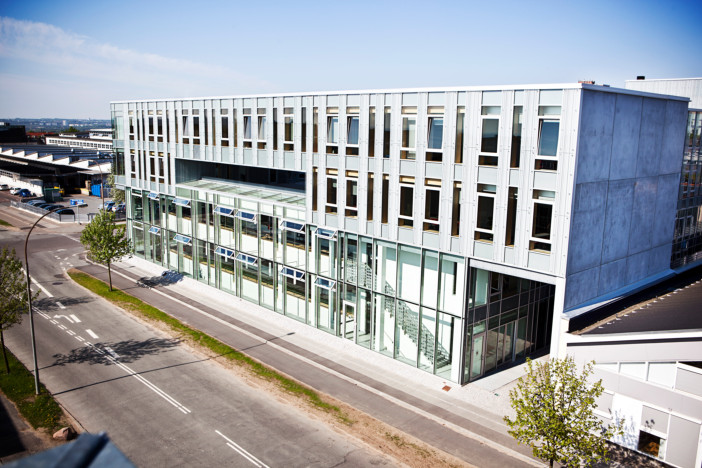
\includegraphics[width=\textwidth]{nygaard_facade.png}
	\end{minipage}
	\hfill
	\begin{minipage}{.48\textwidth}
		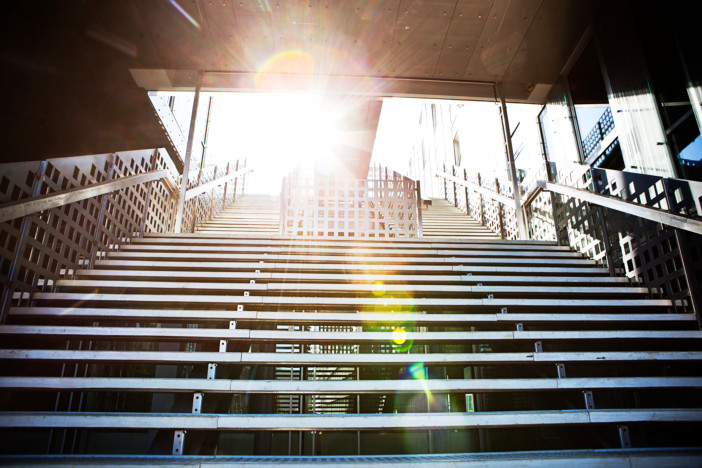
\includegraphics[width=\textwidth]{nygaard_stairs.png}
	\end{minipage}
	\caption{Uncompressed \emph{nygaard\_facade.jpg} and \emph{nygaard\_stairs.jpg} images.}
	\label{fig:uncomp}
\end{figure}

\begin{figure}
	\centering
	\begin{minipage}{.48\textwidth}
		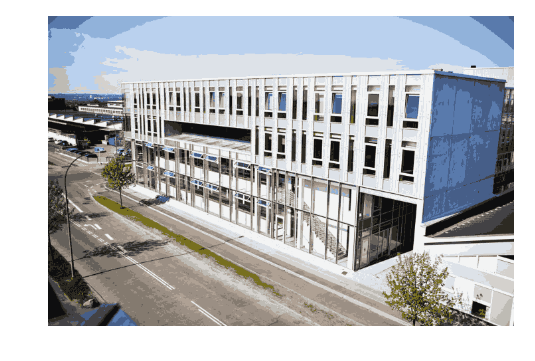
\includegraphics[width=\textwidth]{nygaard_facade_k16.png}
	\end{minipage}
	\hfill
	\begin{minipage}{.48\textwidth}
		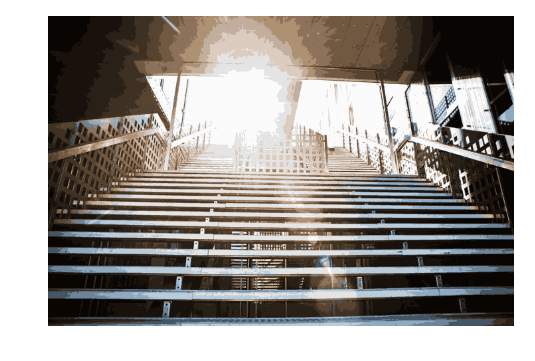
\includegraphics[width=\textwidth]{nygaard_stairs_k16.png}
	\end{minipage}
	\caption{Images with color depth compressed to a set of 16 colors (4bit) with the K-means algorithm.}
	\label{fig:comp16}
\end{figure}

\begin{figure}
	\centering
	\begin{minipage}{.48\textwidth}
		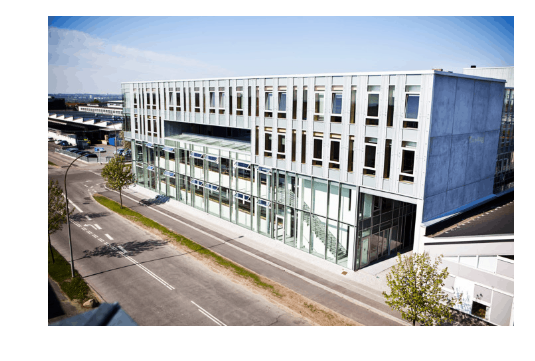
\includegraphics[width=\textwidth]{nygaard_facade_k256.png}
	\end{minipage}
	\hfill
	\begin{minipage}{.48\textwidth}
		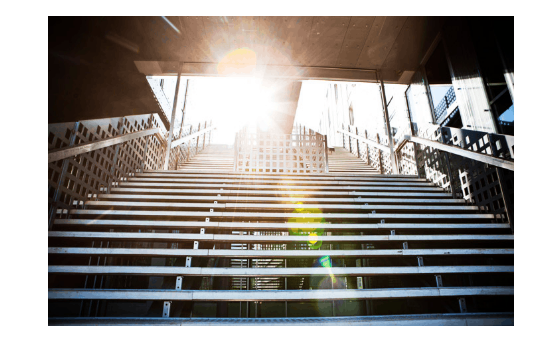
\includegraphics[width=\textwidth]{nygaard_stairs_k256.png}
	\end{minipage}
	\caption{Images with color depth compressed to a set of 256 colors (8bit) with the K-means algorithm.}
	\label{fig:comp256}
\end{figure}

Image quality loss acceptance limit will always be subject to personal taste and dependent on purpose. Compression of images can be done in various ways, and is done most image formats used for photographs. 

\end{document}